
\chapter{石墨烯的生长机理研究}
\section{引言}
    如今,化学气相沉积法已经成为大规模石墨烯生长的主要合成方法。以铜为代表的金属衬底对含碳前驱体的催化作用极大提升了石墨烯的产率。同时,铜衬底自限制效应及较低的碳溶解度抑制了多层石墨烯的生长,提升了石墨烯单层性。尽管如此,由于石墨烯在化学气相沉积法进行生长的过程中通常为多点成核同时生长的方式,所以尽管在铜衬底的表面可以实现单层石墨烯生长,但生长而成的石墨烯通常为多晶的形式,各石墨烯晶畴之间由于生长取向的不同存在晶界。而要实现大面积单层石墨烯单晶的生长,则需要尽可能地扩大单个石墨烯晶畴的面积、尽可能地消除晶界。目前,化学气相沉积法实现大面积石墨烯单晶生长的方式主要有两种。一种是对石墨烯的成核数量进行限制。通过在衬底上实现单点成核,将单晶畴石墨烯缓慢长大的方式实现大面积的单晶石墨烯薄膜。另一种方式是对石墨烯的生长晶向进行调控。通过将多个晶向相同的石墨烯晶畴融合的方式,尽可能地消除石墨烯晶畴之间的晶界,使其能够尽可能完美的形成单晶石墨烯薄膜。相比于限制成核的方式,控制石墨烯生长晶向,使得多点成核的石墨烯畴同时同向生长,更容易实现石墨烯单晶的大规模制备。
    
    由于铜衬底与碳原子较弱的相互作用,石墨烯在铜衬底上的生长方式主要遵循扩散生长机制。在扩散生长机制的作用下,含碳前驱体在铜衬底表面裂解形成具有活性的碳原子,碳原子在铜衬底表面扩散成核生长形成石墨烯晶畴。可以认为,石墨烯的生长过程主要发生在铜衬底的表面,因此理解石墨烯生长过程中和铜衬底表面的作用是理解石墨烯生长机理以及控制石墨烯生长晶向的关键。%//TODO 引用
    
    在\ref{sec:石墨烯优先生长取向}章中,我们使用密度泛函理论,计算了石墨烯在铜衬底表面存在台阶时的优先生长取向。计算结果证明,衬底表面的台阶破坏了原衬底表面的对称性,为石墨烯的成核生长提供了优先生长位点,同时使得石墨烯晶畴的优势生长角度由原来在平坦衬底上非重叠的$\pm 18 ^{\circ}$ 、 $\pm 15 ^{\circ}$坍缩至铜衬底台阶边缘的$\pm 0 ^{\circ}$ 或者 $\pm 30 ^{\circ}$,石墨烯晶畴展现出倾向于单一方向的成核生长。

%//TODO 引言 衬底影响+氧气的影响
\section{计算细节}
    %//TODO vasp 引用等
    在 \ref{sec:石墨烯优先生长取向} 章中,密度泛函理论主要使用 Vienna ab-initio Simulation Package (VASP) 软件包进行计算。由于石墨烯畴$\rm{C_{24}}$与铜衬底均为非磁性体系,出于计算资源的限制,经过测试后我们在 \ref{sec:石墨烯优先生长取向} 章中均采用自旋非极化的计算设置。在密度泛函理论计算中,我们使用广义梯度近似(GGA)下的 Perdew-Burke-Ernzerhof (PBE)泛函描述电子之间的交换关联作用。电子与原子核之间的相互作用采用投影缀加平面波(PAW)赝势。取平面波的截断动能为\SI{400}{\electronvolt}。为了研究铜衬底表面石墨烯的生长情况,我们采用切片模型。在垂直表面方向放置至少\SI{20}{\angstrom}的真空层以防止周期性条件相邻切片的影响。由于切片模型较大的模拟晶胞尺寸,我们在布里渊区中取 $\Gamma$ 点作为积分采样的K空间网络。
%//TODO 石墨烯的生长机理研究 计算细节
\section{衬底晶向对化学气相沉积法生长石墨烯的影响}
\label{sec:石墨烯优先生长取向}
\def\CCluster#1{\rm{C_{#1}}}
    为了探究石墨烯在铜衬底表面的优先生长取向,我们使用碳团簇$\CCluster{24}$作为我们的主要研究对象,考察石墨烯成核生长过程的早期过程中铜衬底表面晶向和台阶的密度对于石墨烯生长方向的影响。对于铜衬底表面晶面结构的选取,我们选择铜(001)以及铜(111)晶面以及以二者为台面的台阶铜表面结构作为研究对象,以覆盖铜衬底表面晶面指数为$\rm{(11n)(n \geqslant 1)}$的情况。
    %\\TODO C24图, Cu(11n)图
    在本章中,我们使用$E_{\rm{f}}$来表征不同生长方向的$\CCluster{24}$团簇在铜衬底表面的形成能。
    \begin{equation}
        E_{\rm{f}}=
        -(E_{\rm{Cu+\CCluster{24}}}-E_{\rm{Cu}}-E_{\rm{\CCluster{24}}})
    \end{equation}
    其中,$E_{\rm{Cu+\CCluster{24}}}$为通过第一性原理计算获得的石墨烯$\CCluster{24}$团簇吸附铜衬底上的总能量,$E_{\rm{Cu}}$为单独铜衬底的能量,$E_{\rm{\CCluster{24}}}$为单独石墨烯$\CCluster{24}$团簇的能量。
    
    对于不同衬底表面上石墨烯$\CCluster{24}$团簇优先生长方向的搜索以及不同生长方向的相对能量计算,我们使用全优化的方式枚举计算不同衬底表面石墨烯$\CCluster{24}$团簇的最优和次优生长方向。为了尽可能搜寻石墨烯$\CCluster{24}$团簇在不同衬底表面的能量最低构型,我们枚举了不同的生长位点,并在每个生长位点上以\SI{6}{\degree}的间隔枚举不同的生长方向。 确定不同衬底表面石墨烯$\CCluster{24}$团簇的最优和次优生长角度后,我们使用线性插值的方式,计算最优和次优生长方向之间的石墨烯$\CCluster{24}$团簇内部的碳原子位置作为中间态。最后,通过固定碳原子XY轴,在Z轴方向优化的方式对这些固定团簇生长角度的中间态进行结构优化,获得石墨烯$\CCluster{24}$团簇在最稳和次稳生长方向之间各个生长角度的形成能$E_{\rm{f}}$。
    %//TODO 计算流程示意图
    \subsection{石墨烯在平坦铜表面的生长晶向}
        我们首先研究石墨烯$\CCluster{24}$团簇在平坦的铜衬底表面的优先生长晶向。如图\ref{GO_001_15_structure}所示,在铜(001)晶面,我们的计算发现当$\CCluster{24}$团簇中央的空洞位于铜衬底表面的面心立方(fcc)位,同时生长角度位15\si{\degree}时,形成能最低。同时,计算获得的$\CCluster{24}$团簇在铜(001)表面的次优生长方向为0\si{\degree},与先前的文献符合\citing{RN692-2015}。从原子结构上看,石墨烯$\CCluster{24}$团簇边缘的碳原子与衬底表面的铜原子具有较强的相互作用。边缘碳原子与衬底表面铜原子的成键使得$\CCluster{24}$团簇的中央拱起,同时也使得$\CCluster{24}$团簇向更多边缘成键的角度旋转,由此在铜(001)表面形成了15\si{\degree}的优先生长方向。

        接着,我们进一步计算了$\CCluster{24}$团簇在铜(001)表面各个角度的相对形成能,结果如图\ref{GO_001_energy}所示。可以看到,$\CCluster{24}$团簇在平坦的铜(001)表面具有两个不重合的能量最小值,分别位于+15\si{\degree}和-15\si{\degree}。$\CCluster{24}$团簇在0\si{\degree}和30\si{\degree}的生长方向处于能量最高值。从能量最高值到能量最低值,$\CCluster{24}$团簇在中间态的相对能量逐渐下降。由于$\CCluster{24}$团簇在旋转至最低能态的过程中不需要越过势垒,因此绝大部分在成核阶段位处于最优生长方向的石墨烯晶畴


        \begin{figure}[ht]
            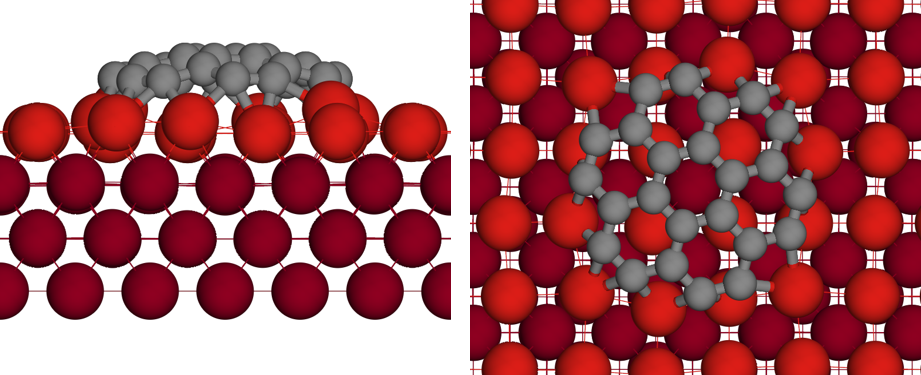
\includegraphics{GO_C24_flat_001_15deg_structure.png}
            \caption{铜(001)晶面石墨烯$\CCluster{24}$团簇的最优生长晶向(\SI{15}{\degree})及原子构型。图中,碳原子为灰色,铜原子为红色,不同层的铜原子以不同亮度进行区分。左侧为侧视图,右侧为俯视图}
            \label{GO_001_15_structure}
        \end{figure}

        \begin{figure}[ht]
            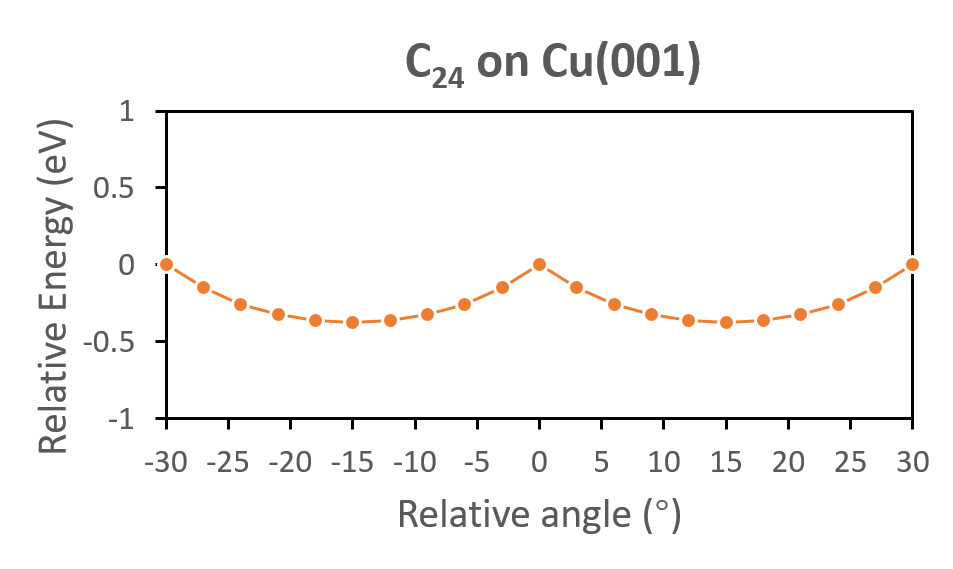
\includegraphics{GO_C24_flat_001_energy.png}
            \caption{铜(001)晶面上不同生长角度的石墨烯$\CCluster{24}$团簇的相对形成能分布。各生长角度相对形成能的参考构型为生长角度0\si{\degree}的构型}
            \label{GO_001_energy}
        \end{figure}
    \subsection{石墨烯在铜表面台阶处的生长晶向}
\section{化学气氛对化学气相沉积法生长石墨烯的影响}
\label{sec:石墨烯氧蚀刻穿透}
    \subsection{化学气相沉积法中石墨烯生长气氛模拟}
    \subsection{氧对石墨烯的穿透蚀刻机制}
    \subsection{氧对石墨烯的穿透生长机制}
    \subsection{氧在石墨烯表面的吸附过程}
    \subsection{氧对石墨烯蚀刻/生长作用的竞争关系及模式切换相图}
\section{总结}

